\documentclass[12pt,a4paper]{article}%
%Options -- Point size:  10pt (default), 11pt, 12pt
%        -- Paper size:  letterpaper (default), a4paper, a5paper, b5paper
%                        legalpaper, executivepaper
%        -- Orientation  (portrait is the default)
%                        landscape
%        -- Print size:  oneside (default), twoside
%        -- Quality      final(default), draft
%        -- Title page   notitlepage, titlepage(default)
%        -- Columns      onecolumn(default), twocolumn
%        -- Equation numbering (equation numbers on the right is the default)
%                        leqno
%        -- Displayed equations (centered is the default)
%                        fleqn (equations start at the same distance from the right side)
%        -- Open bibliography style (closed is the default)
%                        openbib
% For instance the command
%           \documentclass[a4paper,12pt,leqno]{article}
% ensures that the paper size is a4, the fonts are typeset at the size 12p
% and the equation numbers are on the left side

% Tabelas
\usepackage{multirow}

% Símbolos Matemáticos
\usepackage{amsmath}
\usepackage{amsfonts}
\usepackage{amssymb}
\usepackage{bm}
\usepackage{commath}

% Figuras
\usepackage{graphicx}
\usepackage{wrapfig}
\usepackage{float}
\usepackage{subfigure}
\graphicspath{ {img/} }


% Língua e acentos
\usepackage[brazil]{babel}
\usepackage[utf8]{inputenc}
\usepackage[T1]{fontenc}

% Espaçamento
\usepackage[top=3cm, bottom=2cm, left=2cm, right=2cm]{geometry}
\usepackage{indentfirst}

% Pagina em branco
\usepackage{afterpage}
\newcommand \blankpage{
	\null
	\thispagestyle{empty}
	\addtocounter{page}{-1}
	\newpage}

% Lista de códigos
\usepackage{listings}                   % para formatar código-fonte
\lstset{numbers=left, numberstyle=\tiny, stepnumber=1, numbersep=5pt, basicstyle=\scriptsize , frame=trbl}

% Enumerate
\usepackage{enumitem}

% Diagramas
\usepackage{tikz}
\usetikzlibrary{positioning}

\usepackage{gensymb}

%------------------------------------------------------------------------------

\begin{document}

\begin{titlepage}
\begin{center}
\begin{figure}[h]

\includegraphics[scale=0.76]{Imagens/topdotitulo.png}
\end{figure}
\rule{\columnwidth}{1.5mm}
\

\large David Maykon Krepsky Silva\\
\large Daniel Galbes Bassanezi\\

\vspace{4cm}
{\bf \Large Modulador AM}
\vspace{3.5cm}

\begin{flushright}
Data de realização do experimento:\\
20 de agosto de 2015\\
Série/Turma:\\
1000/1011\\
Prof. Dr. Jaime Laelson Jacob 
\end{flushright}

\vspace{3.2cm}
\today

\rule{\columnwidth}{1.3mm}
\end{center}
\end{titlepage}

\newpage

\section{Projeto do controlador no MATLAB}

Função de transferência da planta:
\[
    G(s) = \frac{1}{s^2}
\]

Polos desejados:

\[
    s = -2 \pm 2j
\]


Root Locus sem o compensador:

\begin{figure}[H]
    \centering
    \caption{Root Locus com C(s) = 1.}
    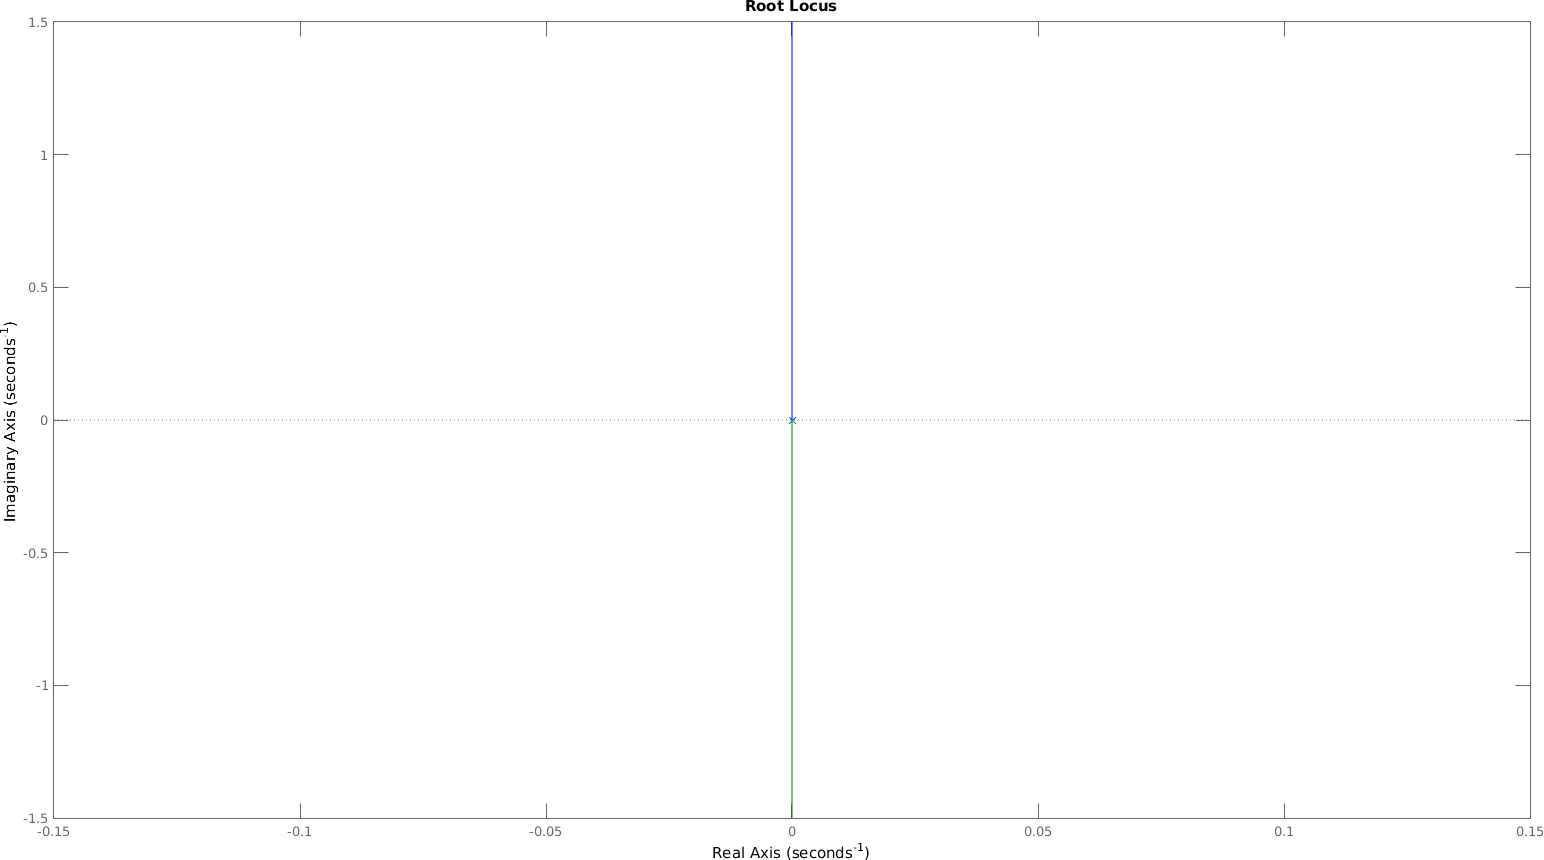
\includegraphics[scale=0.4]{rl_planta}
    \label{f_rl_planta}
\end{figure}


Ganho de fase desejado:
\[
    \Phi = atg-1(\frac{2}{2}) = 45 \degree.
\]

Como são 2 polos na origem, o ganho desejado é $90\degree$;

Calculando o zero e o polo para o compensador por avanço de fase:

\[
    Zero = 1.16
\]

\[
    Polo = 6.76
\]

Através da ferramenta RLTool do MATLAB foi encontrado o ganho do compensador:

\[
    Ganho = 19.0435
\]

A RL de malha fechada do sistema fica:

\begin{figure}[H]
    \centering
    \caption{Root Locus do sistema em malha fechada.}
    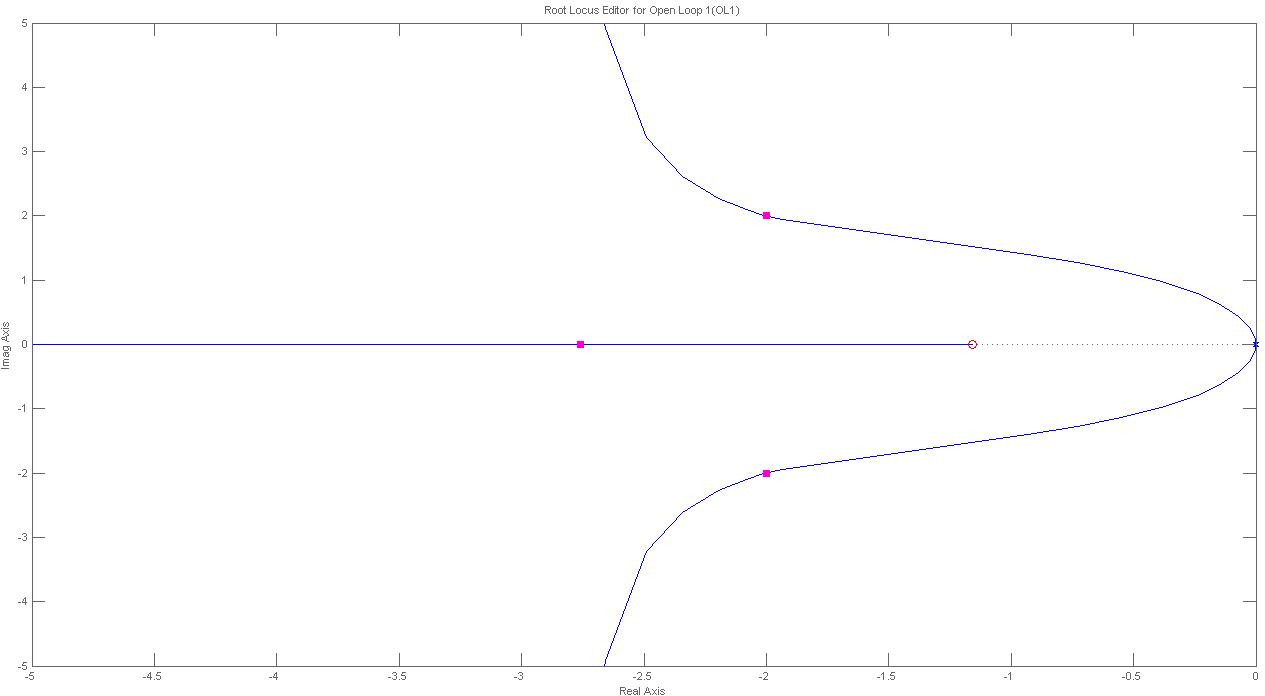
\includegraphics[scale=0.4]{rl}
    \label{f_rl}
\end{figure}

A resposta ao impulso é limitada, ou seja, o controlador é estável.
\begin{figure}[H]
    \centering
    \caption{Resposta ao impulso.}
    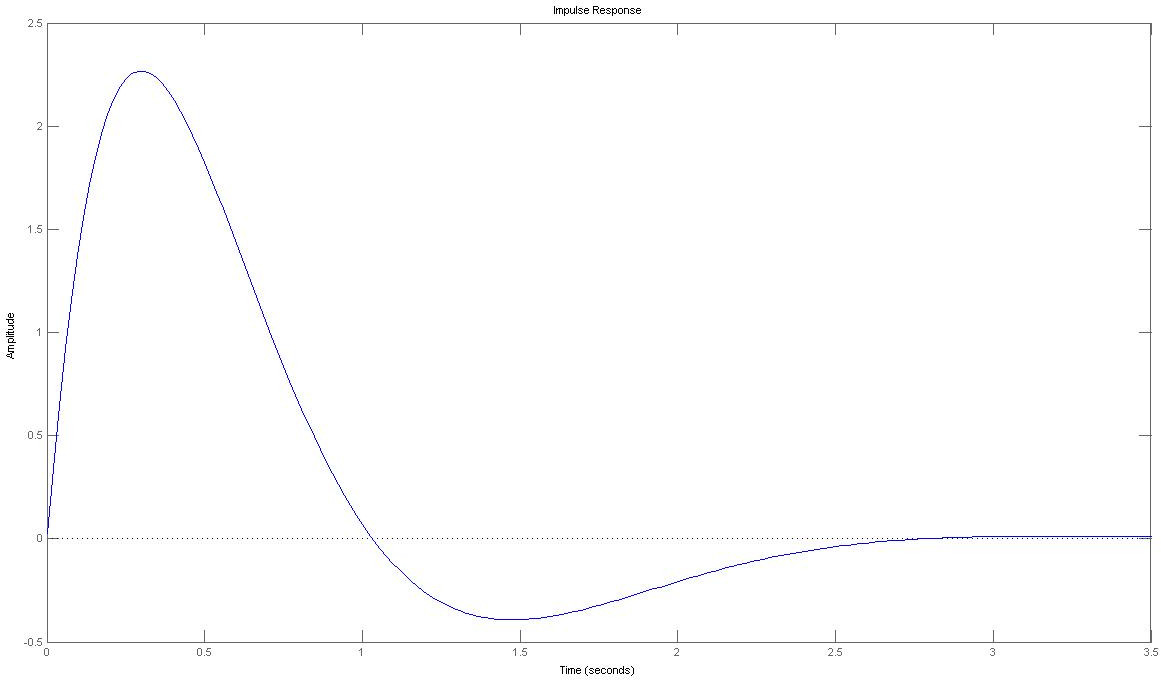
\includegraphics[scale=0.4]{imp}
    \label{f_imp}
\end{figure}

A resposta ao degrau é:
\begin{figure}[H]
    \centering
    \caption{Resposta do sistema a uma entrada do tipo degrau.}
    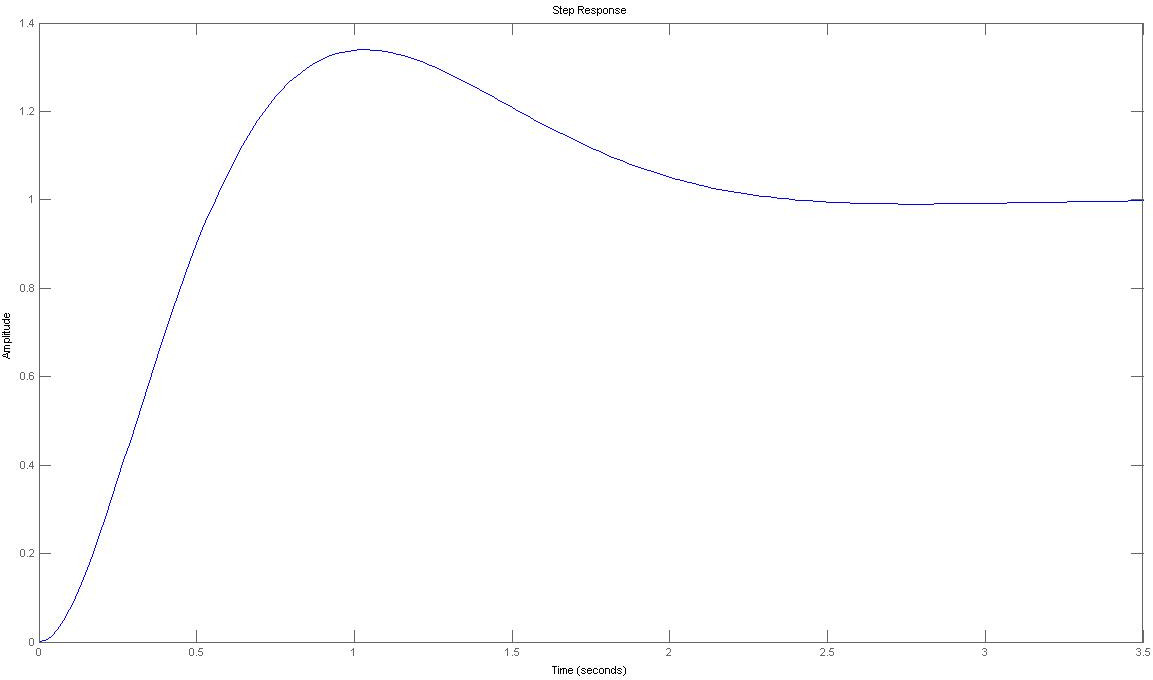
\includegraphics[scale=0.4]{step}
    \label{f_step}
\end{figure}


O circuito do compensador é:
\begin{figure}[H]
    \centering
    \caption{Controlador por avanço de fase feito com ampops.}
    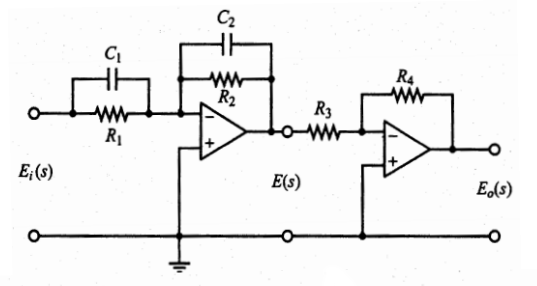
\includegraphics[scale=0.6]{sch_avanco}
    \label{f_sch_avanco}
\end{figure}


Calculando o valor de $R_1$ e $C_1$:

\[
    -\frac{1}{R_1C_1} = 1.16.
\]

Fazendo $R_1$ = $1 k\ohm$.
\[
    C_1 = \frac{1k}{1.16} = 65.5 \, \mu F.
\]


Calculando o valor de $R_2$ e $C_2$:
\[
    -\frac{1}{R_2C_2} = 6.76.
\]

Fazendo $R_2$ = $1 k\ohm$.
\[
C_2 = \frac{1k}{6.76} = 147.93 \, \mu F.
\]

Calculando o valor de $R_3$ e $R_4$:
\[
-\frac{R_4}{R_3} = 19.0435.
\]

Fazendo $R_3$ = $1 k\ohm$.
\[
R_4 = 1k\times 19.0435 = 19.0435  \, k \ohm.
\]

O circuito final montado no ORCAD é:
\begin{figure}[H]
    \centering
    \caption{Circuito do sistema.}
    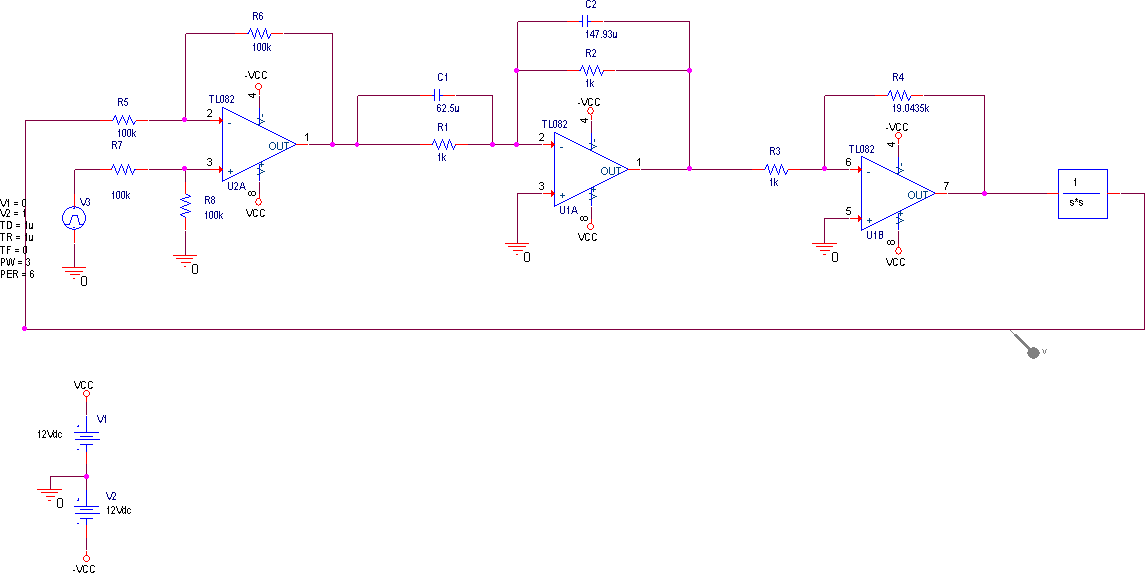
\includegraphics[scale=0.4]{sch}
    \label{f_sch}
\end{figure}

A saída do circuito fica:
\begin{figure}[H]
    \centering
    \caption{Saida do sistema.}
    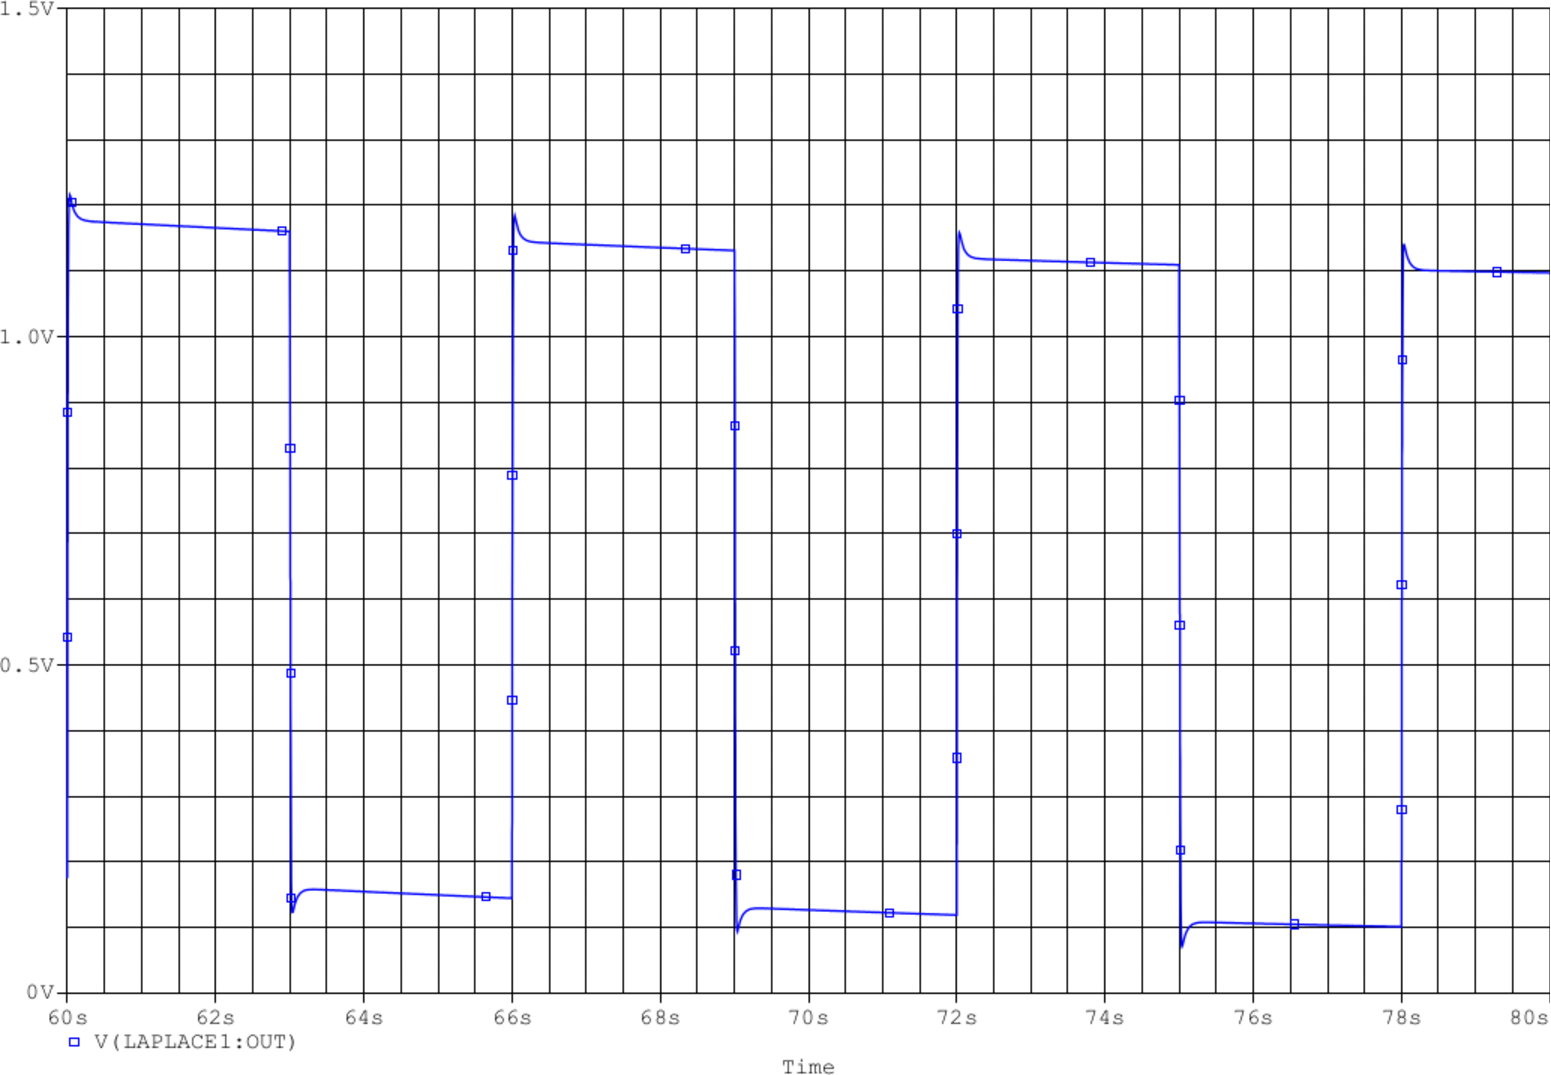
\includegraphics[scale=0.4]{saida}
    \label{f_saida}
\end{figure}

Com zoom:
\begin{figure}[H]
    \centering
    \caption{Zoom na borda.}
    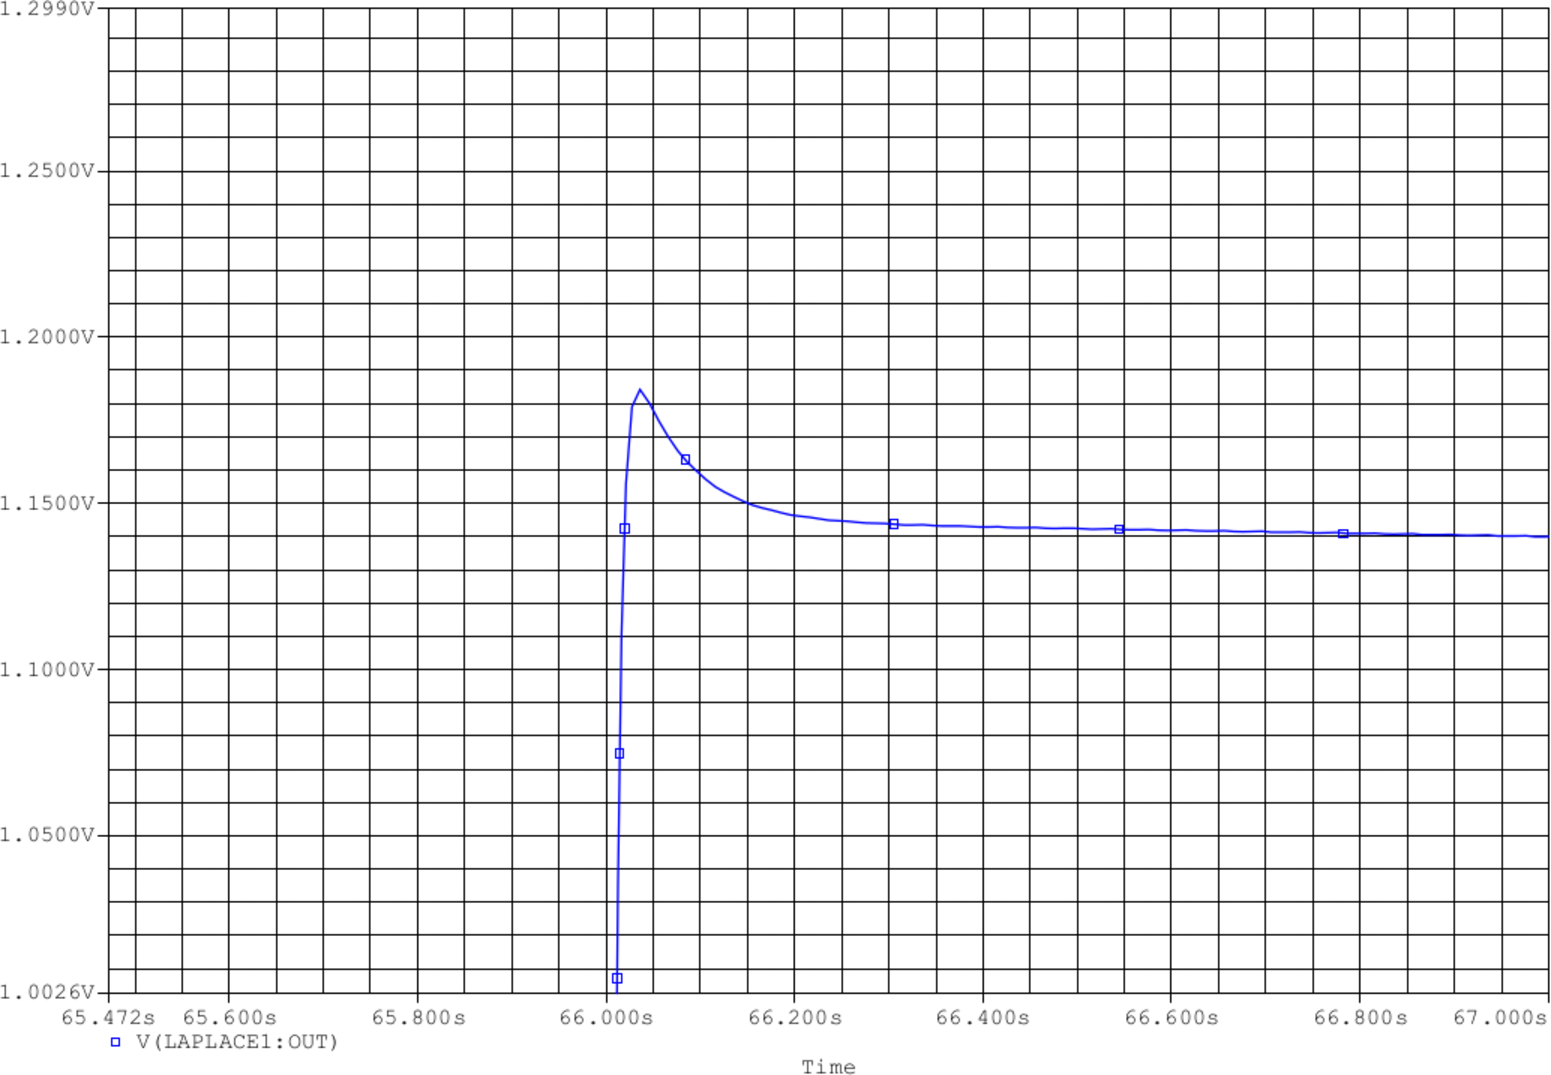
\includegraphics[scale=0.4]{saidazoom}
    \label{f_saidazoom}
\end{figure}


Note que a saída é praticamente igual a do MATLAB.


\end{document}